\documentclass[margin=2mm]{standalone}
%\usepackage{bm}
%\usepackage{calligra}
\usepackage{amsmath} % assumes amsmath package installed
\usepackage{amssymb}  % assumes amsmath package installed
\newcommand{\setfont}[2]{{\fontfamily{#1}\selectfont #2}}
\usepackage{tikz}

\usetikzlibrary{3d}

\usetikzlibrary{calc}
\usetikzlibrary{patterns}
\usetikzlibrary{decorations.text}
\usetikzlibrary{decorations.pathmorphing}
\usetikzlibrary{decorations.markings}
\usetikzlibrary{arrows}
\usetikzlibrary{shapes}

\pgfdeclareimage[width=2.0cm]{VectorFields}{EllipseBetaThird}

\newcommand{\picturefontsize}{\LARGE}
\newcommand{\pictureLineWidth}{0.8mm}

\begin{document}
%!TEX root = ../../14-icra-RealTimeNMPC.tex

\newcommand{\tetazero}{20.55}
\newcommand{\Fkxzero}{-20}
\newcommand{\Fkyzero}{20}

\newcommand{\tetaone}{-20}
\newcommand{\Fkxone}{5}
\newcommand{\Fkyone}{0}

\newcommand{\tetatwo}{20}
\newcommand{\Fkxtwo}{25}
\newcommand{\Fkytwo}{20}

%\includegraphics[width=15cm]{./figures/walking-without-thinking/ConvexHull}
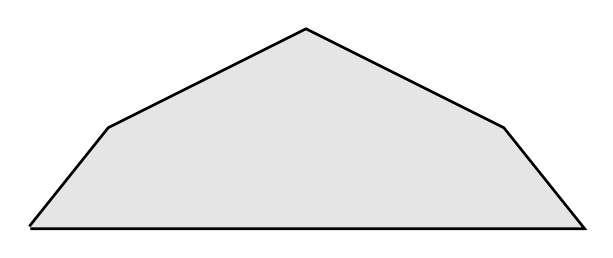
\begin{tikzpicture}[scale=0.125]
\draw [line width=2pt](-28,20)--(-20,30)--(0,40)--(20,30)--(28,20)--(-28,20) node at (-10,30)[black]{} ;
\fill [color=gray!20,line width=2pt] (-28,20)--(-20,30)--(0,40)--(20,30)--(28,20)--(-28,20) ;
\end{tikzpicture}

\end{document}
